\section{整体架构}
该系统的架构需要保证高效的数据处理和实时性能,设计重点包括:

\begin{enumerate}
	\item{模块化设计}
	\par 将整个系统分为若干个独立的模块,例如数据采集模块、数据预处理模块、语义分割模块等。
	这样可以实现各个模块间的解耦,降低系统复杂度,同时提高可维护性和可扩展性。

	\item{流水线并行处理}
	\par 为了提高系统实时性能,可以采用流水线并行处理的方式。这意味着不同的模块可以异步执行(如语义分割和相机位姿估计)。三维重建及语义分割的过程则可以通过GPU加速计算,提高重建速度。

	\item{数据驱动}
	\par 系统应采用数据驱动的方式运行,通过不断地接收、处理、分析RGB-D图像,实现实时三维重建和语义分割,数据流图如图\ref{fig:data_flow}所示。

	\begin{figure}[htb]
		\centering
		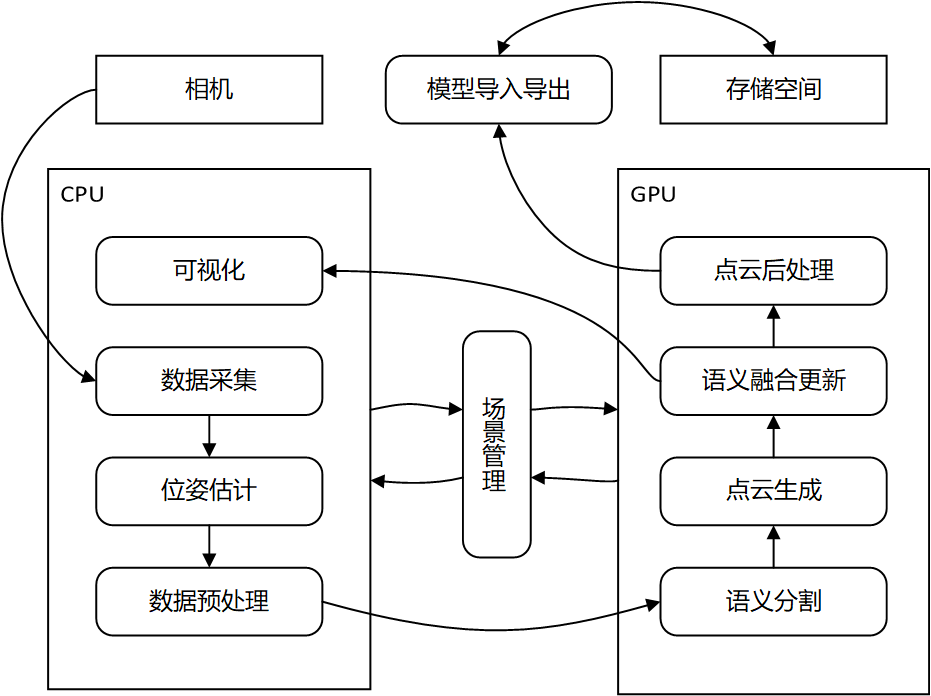
\includegraphics[width=0.9\textwidth]{figures/uml/data_flow.png}
		\caption{数据流图}
		\label{fig:data_flow}
		\note{注:系统的工作流程和数据流向,通过场景管理功能将数据在CPU和GPU之间切换。}
	\end{figure}

	\item{分布式计算}
	\par 根据系统规模和性能要求,可以考虑扩展至多GPU、多核CPU或者集群计算的方式进行处理,这有助于在多个计算节点上分摊计算任务,提高整体处理速度。

	\item{层次化功能划分}
	\par 采用图\ref{fig:architecture}所示的层次化功能划分方法提高系统的灵活性和扩展性。
	从硬件层开始,系统通过与相机、存储空间等硬件设备进行交互,收集和存储数据。
	在系统交互层,数据采集和模型导入导出功能负责管理输入和输出的数据流;用户管理功能负责管理使用系统的所有用户。
	进一步,预处理层包含位姿估计、场景管理、数据预处理和语义分割功能。
	核心算法层为点云生成和语义融合更新功能。
	最后,表现层的点云后处理和可视化功能将处理结果呈现给用户。

	\begin{figure}[htb]
		\centering
		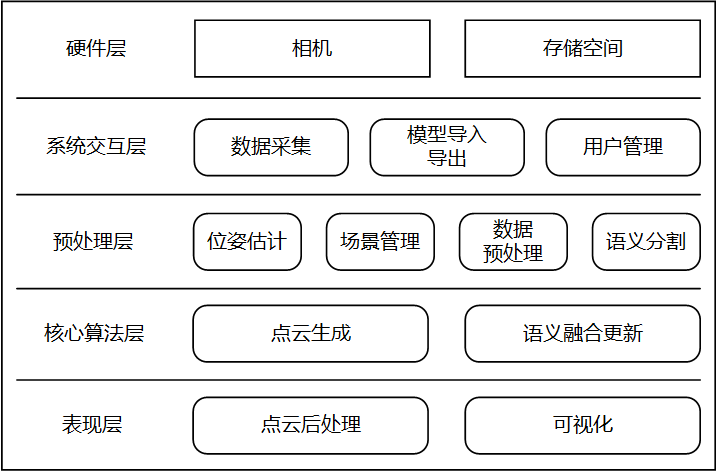
\includegraphics[width=0.8\textwidth]{figures/uml/architect.png}
		\caption{系统架构图}
		\label{fig:architecture}
	\end{figure}

	\item{用户界面与可视化}
	\par 设计易用的用户界面,实时展示重建结果和语义分割结果,便于观察与调试。
\end{enumerate}

\par 不难看出,上述理念被充分地应用在了模型、视图模型和视图这三个层次,因此,本系统可以采取MVVM(Model-View-ViewModel)架构模式。

\begin{figure}[htb]
	\centering
	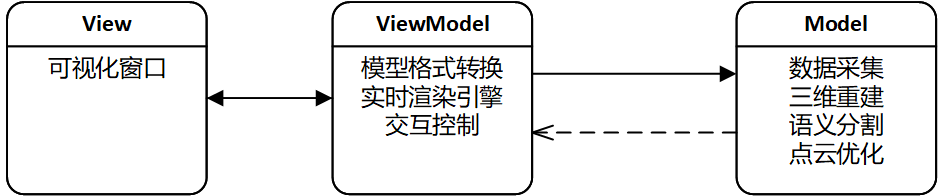
\includegraphics[width=0.9\textwidth]{figures/uml/mvvm_pattern.png}
	\caption{MVVM 模式架构}
	\label{fig:mvvm_pattern}
\end{figure}

\par 如图\ref{fig:mvvm_pattern}所示,Model(模型)负责处理核心业务逻辑,包括数据采集、三维重建和语义分割等。ViewModel(视图模型)负责处理数据逻辑,将模型中的数据转换为适合视图展示的格式。
另外,视图模型还可以处理视图中的用户操作,例如调整参数、控制重建和分割过程等。View(视图)负责实时显示三维重建和语义分割的结果,同时提供用户操作界面。

\par 该系统采用MVVM模式有以下好处:

\begin{enumerate}
	\item{解耦性}
	\par MVVM模式明确地将系统分为三个部分,这种分层架构有助于降低各个模块之间的耦合度,使它们相互独立,便于维护和升级。

	\item{可维护性}
	\par 由于MVVM模式中各个模块的职责分离,系统开发过程中可以更容易地定位和修复问题,从而提高系统的可维护性。同时,当需求发生变化时,可以在不影响其他组件的情况下单独更新某个模块。

	\item{数据绑定}
	\par MVVM模式支持数据绑定,使得ViewModel可以自动将重建完成的点云数据更新传递给View,减少数据同步的代码量,降低出错概率。

	\item{重用性}
	\par 在MVVM模式下,ViewModel可以在不同的View中重用(如语义动画、实例动画)。这意味着当需要在多个视图中显示相似的数据时,可以避免重复编写代码。
\end{enumerate}